% % % % % % % % % % % % % % % % % % % % % % % % % % % % % % % % % % % % % % % % % % % %
%                                                                                     %
% Short Sectioned Assignment LaTeX Template Version 1.0 (5/5/12)                      %
% This template has been downloaded from: http://www.LaTeXTemplates.com               %
%                                                                                     %
% Original author:  Frits Wenneker (http://www.howtotex.com)                          %
%                                                                                     %
% Modified by: Fco Javier Sueza Rodríguez (fcosueza@disroot.org)                      %
%                                                                                     %
% Changes:                                                                            %
%	    - Custom Chapters, Sections and Subsections (titlesec package)                %
%           - Document type scrbook (oneside)                                         %
%           - Use babel-lang-spanish package and marvosym                             %
%           - Use hyperref, enumitem, tcolorbox and glossaries packages               %
%           - Use Time New Roman (mathptmx), Helvetic and Courier fonts               %
%                                                                                     %
% License: CC BY-NC-SA 3.0 (http://creativecommons.org/licenses/by-nc-sa/3.0/)        %
%                                                                                     %
% % % % % % % % % % % % % % % % % % % % % % % % % % % % % % % % % % % % % % % % % % % %

%-----------------------------------------------%
%	              Packages                  %
%-----------------------------------------------%

\documentclass[paper=a4, fontsize=11pt, oneside]{scrbook}

% ---- Text Input/Output ----- %

\usepackage[T1]{fontenc}
\usepackage[utf8]{inputenc}
\usepackage{mathptmx}
\usepackage[scaled=.92]{helvet}
\usepackage{courier}
\usepackage[indent=12pt]{parskip}

\usepackage{geometry}
\geometry{verbose,tmargin=3cm,bmargin=3cm,lmargin=2.6cm,rmargin=2.6cm}

% ---- Language ----- %

\usepackage[spanish]{babel}
\usepackage{marvosym}

% ---- Another packages ---- %

\usepackage{amsmath,amsfonts,amsthm}
\usepackage{graphics,graphicx}
\usepackage{titlesec}
\usepackage{fancyhdr}
\usepackage{tcolorbox}
\usepackage{hyperref}
\usepackage{enumitem}
\usepackage[automake]{glossaries}

%--------------------------------------------------------------------%
%                      Customizing Document                          %
%--------------------------------------------------------------------%


% ----------- Custom Chapters, Sections and Subsections -------------- %

\titleformat{\chapter}[display]
			{\bfseries\Huge}
			{Tema \ \thechapter} {0.5ex}
			{\vspace{1ex}\centering}

\titleformat{\section}[hang]
			{\bfseries\Large}
			{\thesection}{0.5em}{}

\titleformat{\subsection}[hang]
			{\bfseries\large}
			{\thesubsection}{0.5em}{}

\titleformat{\subsubsection}[hang]
			{\bfseries\large}
			{\thesubsubsection}{0.5em}{}

\hypersetup{
    colorlinks=true,
    linkcolor=black,
    urlcolor=magenta
}

% ------------------- Custom heaaders and footers ------------------- %

\pagestyle{fancyplain}

\fancyhead[]{}
\fancyfoot[L]{}
\fancyfoot[C]{}
\fancyfoot[R]{\thepage}

\renewcommand{\headrulewidth}{0pt} % Remove header underlines
\renewcommand{\footrulewidth}{0pt} % Remove footer underlines

\setlength{\headheight}{13.6pt} % Customize the height of the header

% --------- Numbering equations, figures and tables ----------------- %

\numberwithin{equation}{section} % Number equations within sections
\numberwithin{figure}{section} % Number figures within sections
\numberwithin{table}{section} % Number tables within sections

% ------------------------ New Commands ----------------------------- %

\newcommand{\horrule}[1]{\rule{\linewidth}{#1}} % Create horizontal rule command


%----------------------------------------------------------------------------------------
%	TÍTULO Y DATOS DEL ALUMNO
%----------------------------------------------------------------------------------------

\title{
\normalfont \normalsize
\textsc{{\bfseries Curso 2022-2023} \\ Ciclo Superior de Desarrollo de Aplicaciones Web \\ IES Aguadulce} \\ [25pt]
\horrule{0.5pt} \\[0.4cm]
\huge Lenguajes de Marcas y Sistemas de Gestión de la Información\\
\horrule{0.5pt} \\[0.4cm]
}

\author{Francisco Javier Sueza Rodríguez}
\date{\normalsize\today}

%----------------------------------------------------------------------------------------
%                                     DOCUMENTO
%----------------------------------------------------------------------------------------

\makeglossaries
\loadglsentries{glossary.tex}

\begin{document}

\maketitle

\newpage

\tableofcontents

\listoffigures

%\listoftables

\newpage
\chapter{Lenguajes de Marcas y Sistemas de Gestión de la Información}
En esta unidad vamos a estudiar los aspectos básicos de los lenguajes de marcas y los sistemas de gestión de la información. Por un lado, veremos la evolución de los \textbf{lenguajes de marcas}, desde GML hasta HTML, así como sus elementos y atributos, haciendo especial énfasis en XML. A continuación, veremos en que consisten los \textbf{sistemas de gestión de la información}, en concreto los \textbf{ERP}, sus características, configuración básica, personalización,..etc.

\section{Definición y Clasificación de los Lenguajes de Marcas}
Los <<lenguajes de marcas>> sirven para \textbf{codificar un documentos}. Estos incorporan \textbf{etiquetas} o marcas con \textbf{información adicional} sobre como se estructura el texto o como se presenta. El lenguaje de marcas será el que defina que etiquetas se permiten, donde deben colocarse y que significado tienen.

Todo lenguaje de marcas esta definido en un documento denominado \textbf{\gls{DTD}}, donde se establecen las marcas, los elementos utilizados por dicho lenguaje y sus correspondientes etiquetas y atributos, así como su sintaxis.

Los lenguajes de marcas se pueden clasificar, principalmente, en tres grupos:

\begin{itemize}
    \item \textbf{Orientados a la presentación}: son los utilizados generalmente por los procesadores de texto y definen como debe presentarse el documento, es decir, el formato que tiene.
    \item \textbf{De procedimientos}: orientados también a la presentación, pero en este caso, dentro de un \textbf{marco procedural} que permite la definición de macros, es decir, el programa que representa el documento debe interpretar el código en el mismo orden que aparece. Algunos ejemplos son \textbf{TeX}, \textbf{LaTeX} y \textbf{Postscript}
    \item \textbf{Descriptivos o semánticos}: estos lenguajes no describen la presentación del documento, sino que \textbf{describen la información}, que es lo que se esta representando sin especificar como debe presentarse.
\end{itemize}

Algunos ejemplos de lenguajes de marcado agrupados por su ámbito de uso son los siguientes:

\begin{itemize}
    \item \textbf{Documentación Electrónica}:
    \begin{itemize}
        \item \textbf{RTF} (Rich Text Format): fue desarrollado por Microsoft en 1987 y permite el intercambio de documentos entre los diferentes procesador de texto.
        \item \textbf{TeX}: creado por \href{https://es.wikipedia.org/wiki/Donald_Knuth}{Donald Knuth}, este lenguaje esta especialmente enfocado en la creación de textos científicos. Es considerado la mejor forma de componer formulas matemáticas complejas. \cite{tex}
        \item \textbf{Wikitexto}: permite la creación de páginas wiki en servidores preparados para soportar este lenguaje.
        \item \textbf{DocBook}: permite generar documentos separando la estructura lógica del documento de su formato, permitiendo que estos documentos puedan publicarse en diferentes formatos sin tener que modificar el documento original.
    \end{itemize}
    \item \textbf{Tecnologías de Internet}:
    \begin{itemize}
        \item \textbf{HTML},\textbf{XHTML} (Hypertext Markup Language, eXtensible Hypertext Markup Language): estos lenguajes están orientados a la creación de páginas web.
        \item \textbf{RSS} (Really Simple Sindication): permite la difusión de contenido web mediante la sindicación de contenidos.
    \end{itemize}
    \item Otros lenguajes especializados:
    \begin{itemize}
        \item \textbf{MathML} (Mathematica Markup Language): especializado en expresar los formalismos matemáticos de forma que puedan ser entendidos por diferentes aplicaciones.
        \item \textbf{VoiceXML} (Voice eXtended Markup Language): permite el intercambio de información entre usuarios y una aplicación con capacidad de reconocer el habla.
        \item \textbf{MusicXML}: permite el intercambio de partituras entre diferentes editores de partituras.
    \end{itemize}
\end{itemize}

\section{Evolución de los Lenguajes de Marcas}
A finales de los \textbf{años 60} surgen unos lenguajes informáticos, diferentes de los lenguajes de programación, orientados a la gestión de la información. Con el desarrollo de los editores y procesadores de texto surgen los primeros lenguajes informáticos orientados a la descripción y estructuración de la información: \textbf{los lenguajes de marcas}. Paralelamente también surgen otros lenguajes orientados a la representación, almacenamiento y consultar de grandes cantidades de datos: lenguajes y sistemas de bases de datos.

Los lenguajes de marcas surgieron inicialmente como lenguajes formados por un conjunto de códigos que los procesadores de textos insertaban en los documentos para dirigir el proceso de presentación (impresión) mediante una impresora. Al igual que los lenguajes de programación, estos estaban \textbf{ligados} a las características de los \textbf{procesadores de texto}y las \textbf{impresoras} en los que se usaban y no permitían a los programadores abstraerse de dichas características.

Posteriormente se añadió como medio de presentación a la pantalla y se automatizó el proceso, teniendo ya solo que pulsar una combinación teclas para lograr los resultados deseados en vez de hacerlo a mano. Este marcado estaba orientado exclusivamente a la presentación de la información, aunque posteriormente se le dieron nuevos uso surgiendo con ello el \textbf{formato generalizado}.

\subsection{El origen: GML y SGML}
Uno de los problemas que ha tenido la informática ha sido la \textbf{falta de estandarización} en los formatos de información usados por los diferentes programas.

En los años 60, \textbf{IBM} encargo a \textbf{Charles F. Goldfarb} la construcción de un sistema de edición, almacenamiento y búsqueda de documentos legales. Después de analizar el funcionamiento de la empresa se llego a la conclusión de que necesitaban un formato estándar a todos los departamentos para gestionar la documentación.

Así fue como se creó \textbf{\gls{GML}}, un formato que permitía describir los documentos de tal forma que el resultado fuese independiente de la plataforma o la aplicación utilizada. Este formato evolucionó hasta que en 1986 se creó el estándar \textbf{ISO 8879} donde se especificaba el formato \textbf{\gls{SGML}}, un lenguaje muy complejo y que requería de unas herramientas de software caras, por lo que su uso quedó relegado a grandes aplicaciones industriales.


\begin{figure}[h]
    \begin{tcolorbox}[sharp corners, colback=yellow!30, colframe=white!20]
      \scriptsize
      \begin{verbatim}
<email>
    <remitente>
        <nombre>Peter</nombre>
        <apellido>Pan</apellido>
    </remitente>
    <destinatario>
        <direccion>campanilla@paisdenuncajamas.com</direccion>
    </destinatario>
    <asunto>Paseo</asunto>
    <mensaje>¿Te apetece dar una vuelta?</mensaje>
</email>
      \end{verbatim}
    \end{tcolorbox}
\caption{Documento SGML simple}
\end{figure}

\subsection{La Popularización: HTML}

En 1990, \href{https://es.wikipedia.org/wiki/Tim_Berners-Lee}{\textbf{Tim Berners-Lee}} creó el World Wide Web y conociendo SGML, se encontró con la necesidad de compatibilizar, enlazar y organizar gran cantidad de documentos procedentes de diversos sistemas. Como solución, a partir de la sintaxis de SGML, creó un lenguaje de descripción de documentos llamado \textbf{\gls{HTML}}, combinando dos estándares ya existentes:

\begin{itemize}
    \item \textbf{\gls{ASCII}}: código basado en el alfabeto latino, tal como se usa en inglés moderno \cite{ascii}. Cualquier procesador de textos simple puede reconocer y almacenar este formato, permitiendo la transferencia de datos entre dos ordenadores.
    \item \textbf{SGML}: lenguaje que permite dar estructura al texto aplicando diferentes formatos.
\end{itemize}

\textbf{HTML} es una \textbf{versión simplificada de SGML}, ya que solo utiliza las instrucciones absolutamente necesarias. Gracias a su simplicidad, tuvo un éxito rotundo en la World Wide Web, convirtiéndose rápidamente en el \textbf{estándar general} para la \textbf{creación de páginas web}. Actualmente, HTML es el tipo de documento más utilizado en el mundo.

\begin{figure}[h]
    \begin{tcolorbox}[sharp corners, colback=yellow!30, colframe=white!20]
        \scriptsize
        \begin{verbatim}
<!DOCTYPE HTML>
<html>
    <head>
        <meta charset="utf-8" />
        <title>Ejemplo1</title>
    </head>
    <body>
        <p>Párrafo de ejemplo</p>
    </body>
</html>
        \end{verbatim}
    \end{tcolorbox}
    \caption{Documento HTML simple}
\end{figure}

\subsection{La Madurez: XML}
Uno de los problemas que surgió con HTML es que la cantidad de documentos escritos en este lenguaje creció exponencialmente, muchos de los cuales no se ceñían a ningún estándar generando bastante caos. Como respuesta es ese problema, el \textbf{\gls{W3C}} estableció en 1998 el estándar internacional \textbf{\gls{XML}}, un lenguaje de marcas puramente estructural, que \textbf{no incluye información sobre el diseño}, y permite la creación de etiquetas adaptadas a las necesidades, convirtiéndose con rapidez en el estándar para intercambio de datos en la web.

\textbf{XML} es un \textbf{\gls{metalenguaje}} con las siguientes características:

\begin{itemize}
    \item Permitir definir etiquetas propias.
    \item Permitir asignar atributos a las etiquetas.
    \item Utilizar un esquema para definir de forma exacta las etiquetas y sus atributos.
    \item La estructura y el diseño son independientes.
\end{itemize}

En realizad XML es un \textbf{conjunto de estándares} relacionados entre sí y que comprende los siguientes:

\begin{itemize}
    \item \textbf{XLS} (eXtensible Style Language): permite definir hojas de estilo para XML e incluye capacidad de transformación de documentos.
    \item \textbf{XML Linking Language}: determina aspectos sobre los enlaces entre documentos XML e incluye \textbf{Xpath}, \textbf{Xlink} y \textbf{Xpointer}.
    \item \textbf{XML Namespaces}: proveen de un contexto donde se aplican las marcas del documento XML y que se diferencian de otras con el mismo nombre válidas en otros contextos.
    \item \textbf{XML Schemas}: permiten definir restricciones que se aplicarán a un documento XML. Actualmente las mas utilizadas son \textbf{DTD}.
\end{itemize}


\begin{figure}[h]
    \begin{tcolorbox}[sharp corners, colback=yellow!30, colframe=white!20]
      \scriptsize
      \begin{verbatim}
<?xml version="1.0" encoding="UTF-8xºx"?>
<!DOCTYPE biblioteca>

<biblioteca>
    <ejemplar tipo="libro" isbn="978-2-7460-4958-1" edicion="1">
        <titulo>XML practico</titulo>
        <editorial>Ediciones Eni</editorial>
        <autor>Sebastien Lecomte</autor>
        <autor>Thierry Boulanger</autor>
        <autor funcion="traductor">Ángel Belinchon Calleja</autor>
        <prestamos>
            <lector inicio="13/05/2014" devolucion="15/05/2014">Pedro López</lector>
            <lector inicio="13/07/2015" devolucion="15/07/2015">Ali Méndez</lector>
        </prestamos>
     </ejemplar>
</biblioteca>
      \end{verbatim}
    \end{tcolorbox}
    \caption{Documento XML simple}
\end{figure}

\subsection{Comparación XML y SGML}
Aunque XML esta basado en SGML, estos tienen muchas diferencias. A continuación se muestra una tabla con las principales diferencias de estos dos lenguajes de marcas.

 \begin{table}[h]
     \centering
    {\renewcommand{\arraystretch}{1.5}
        \begin{tabular}[c]{ |l|l| }
            \hline
            \multicolumn{1}{|c|}{\textbf{XML}} & \multicolumn{1}{|c|}{\textbf{SGML}} \\ \hline
            Su uso es sencillo & Su uso es my complejo \\ \hline
            Trabaja con documentos bien formados & Solo Trabaja con documentos válidos \\ \hline
            Desarrollo de aplicaciones a bajo coste & Aplicaciones para procesarlo costosas \\ \hline
            Muy utilizado en informática y otras áreas & Se utiliza en sectores muy específicos\\ \hline
            Compatibilidad e integración con HTML & No hay compatibilidad con HTML \\ \hline
            Formateo y estilos fáciles de aplicar & Formateo y estilo relativamente complejos \\ \hline
    \end{tabular}}
 \end{table}

Como vemos en esta tabla, SGML es un un lenguaje mas complejo y costoso que XML, además de imponer mas restricciones, haciéndolo un lenguaje menos flexible que XML y mas orientado a sectores concretos. Para obtener más información sobre XML, podemos consultar el \href{https://www.w3.org/TR/REC-xml/}{Estándar XML} publicado por la W3C.

\subsection{Comparación XML y HTML}
Aunque tanto XML como HTML se crearon a partir de SGML y su sintaxis es similar, son lenguajes diferentes con propósitos diferentes, como podemos ver en la siguiente tabla.

 \begin{table}[h]
    \centering
    {\renewcommand{\arraystretch}{1.5}
        \begin{tabular}[c]{ |l|l| }
            \hline
            \multicolumn{1}{|c|}{\textbf{XML}} & \multicolumn{1}{|c|}{\textbf{HTML}} \\ \hline
            Es un perfil de SGML & Es una aplicación de SGML \\ \hline
            Permite definir conjuntos de etiquetas & Aplica un conjunto limitado de etiquetas \\ \hline
            Modelo de hiperenlaces complejo & Modelo de hiperenlaces simple \\ \hline
            Navegador como plataforma de desarrollo & Navegador como visor de páginas \\ \hline
            Compatibilidad e integración con HTML & No hay compatibilidad con HTML \\ \hline
            Fin de las etiquetas propietarias & Problema de la no compatibilidad en navegadores \\ \hline
    \end{tabular}}
\end{table}

\section{Etiquetas, Elementos y Atributos}
Los lenguajes de marcas usan una serie de etiquetas intercaladas en un documento sin formato, las cuales serán posteriormente por el interprete del lenguaje.

Existen tres términos ampliamente utilizados en los lenguajes de marcas:

\begin{itemize}
    \item \textbf{Etiquetas}: una etiqueta, también llamada \textbf{tag}, es un pequeño bloque de código que se escribe encerrado entre los símbolos \textbf{menor que} (\textbf{<}) y \textbf{mayor que} (\textbf{>}). Normalmente se utilizan \textbf{dos etiquetas}, una de \textbf{inicio} y otra de \textbf{fin}, para indicar que el efecto que queríamos conseguir ha finalizado, con la única diferencia que a la etiqueta de fin se le añade el carácter \textbf{/} antes del nombre.
    \item \textbf{Elemento}: representan estructuras mediante las que se organiza el contenido del documento, o acciones que se desencadenan cuando el navegador lo interpreta. Está \textbf{compuesto} de la \textbf{etiqueta de apertura}, la \textbf{etiqueta de cierre} y el \textbf{contenido entre ambas}.
    \item \textbf{Atributo}: es un par \textbf{nombre-valor}, que se encuentra al inicio de un elemento e indican diferentes propiedades asociadas a ese elemento
\end{itemize}

\begin{figure}[h]
    \centering
    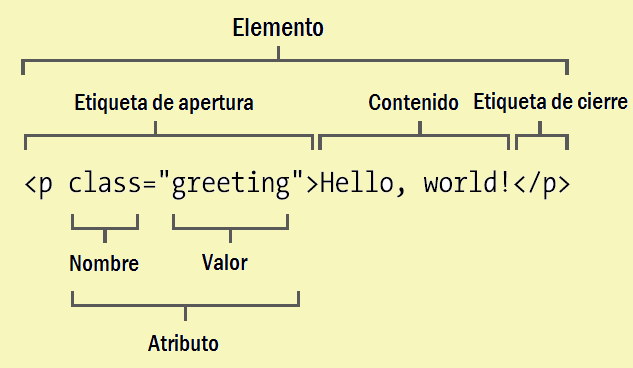
\includegraphics[scale=0.50]{elemento-HTML.png}
    \caption{Partes de un elemento HTML}
\end{figure}

\section{Herramientas de Edición}
Para trabajar con XML es necesario, por un lado, editar los documentos, y por otro procesarlos. Por ello, necesitaremos dos tipos de herramientas para trabajar con él, estas son:

\begin{itemize}
    \item \textbf{Editores XML}

    Una característica de los lenguajes de marcas es que se basan en la utilización de ficheros de \textbf{\gls{texto plano}}, por lo que basta con usar cualquier editor de texto para construir un documento XML.

    Aunque podemos usar cualquier editor, cuando elaboramos documentos XML complejos es conveniente usar
    algún software de edición XML. Estos nos ayudan a crear estructuras y etiquetas de los elementos usados en XML, resaltan las etiquetas para diferenciarlas más cómodamente y ademas incluyen ayudas para la creación de otros elementos como DTD, hojas de estilo CSS o XLS,.. El W3C ha desarrollado un editor HTML, XHTML, CSS y XML gratuito llamado Amaya, pero existen otros muchos gratuitos como: Notepad++, VSCode, Sublime Text, Netbeans,..etc

    \item \textbf{Procesadores XML}

    Para interpretar un documento XML puede usarse cualquier navegador. Los procesadores XML permiten visualizar los documentos XML y acceder a su contenido y estructura. Un \textbf{procesador} es un conjunto de módulos de software entre los que se encuentra un \textbf{parser}, que comprueba que el documento cumple las normas establecidas para que pueda abrirse. Estás normas pueden corresponderse a las necesarias para trabajar con documentos de tipo válido o solo exigir que el documento este bien formado. A los primeros se le conocen como \textbf{procesadores validadores} y a los segundos como \textbf{procesadores no validadores}.

    Para publicar documentos XML en internet se usan \textbf{procesadores XSLT}, que permiten generar archivos HTML a partir de XML.

    Puesto que XML se usa para el intercambio de archivos entre aplicaciones, hay que recurrir a motores independientes como <<XML para Java>> de IBM, JAXP de Sun, etc
\end{itemize}

\section{XML}
\textbf{XML}, que significa \textit{eXtensible Markup Language}, es un lenguaje que permite definir lenguajes de marcas desarrollado por el W3C y utilizado para almacenar datos de forma legible. Proviene del lenguaje SGML y permite definir la gramática de lenguajes específicos para estructurar documentos. \cite{xml}

Su importancia radica en que permite \textbf{compartir datos} entre diferentes equipos y aplicaciones de forma \textbf{segura}, \textbf{fiable} y \textbf{sencilla}. El hecho de que diferentes equipos y aplicaciones puedan leer y generar archivos en este formato lo convierte en una herramienta muy útil para el envío de información a través de la Web. Aunque a veces suele confundirse con HTML, podemos decir que HTML esta diseñado para mostrar datos en nuestras pantallas mientras que XML esta diseñado para almacenar y compartir esos datos.

El XML ahorra tiempos de desarrollo y proporciona ventajas, dotando a webs y aplicaciones de un método muy potente para almacenar y compartir información. Por ello, se ha convertido en un formato universal usado por todo tipo de sistemas operativos y dispositivos.

\subsection{Estructura y Sintaxis}
Un documento XML es un documento de de texto, con la \textbf{extensión .xml}, compuesto de un \textbf{conjunto de etiquetas}, \textbf{estructuradas en árbol}, que describen la organización del documento y que es interpretado por un navegador Web.

La \textbf{características básicas} de XML son las siguientes:

\begin{itemize}
    \item Es directamente \textbf{compatible} con protocolos usados en en la Web como \textbf{HTTP} y \textbf{URL}.
    \item Todo documento que verifique las reglas de XML esta \textbf{conforme con SGML}.
    \item \textbf{No se requieren conocimientos de programación} para realizar tareas sencillas en XML.
    \item Los documentos XML son\textbf{ fáciles de crear}.
    \item \textbf{La difusión} de documentos XML \textbf{está asegurada}, ya que cualquier procesador de XML puede leer documentos XML.
    \item El marcado de XML es \textbf{legible para los humanos}.
    \item El diseño de XML es \textbf{formal y conciso}.
    \item XML es \textbf{extensible}, \textbf{adaptable} y \textbf{aplicable} a una gran variedad de situaciones.
    \item XML es \textbf{orientado a objetos}
    \item Todo documento XML se \textbf{compone} de \textbf{datos de marcado} y \textbf{datos carácter} entremezclados.
\end{itemize}

El \textbf{proceso de creación} de un documento pasa por varias etapas en las que el éxito de cada una de ellas se basa en la calidad de la anterior. Estas etapas son:

\begin{enumerate}
    \item Especificación de requisitos.
    \item Diseño de etiquetas.
    \item Marcado de los documentos.
\end{enumerate}

El \textbf{marcado} son etiquetas que se añaden para estructurar los documentos y permitir a los ordenadores interpretar los textos. Los \textbf{datos carácter} son los que componen la verdad información del documento.

Los documentos XML también pueden \textbf{contener comentarios}, que son interpretados por el intérprete XML y que comienzan con la cadena \textit{<!--} y finalizan con \textit{-->}. Pueden estar en cualquier posición del documento salvo en:

\begin{itemize}
    \item El prólogo
    \item Dentro de una etiqueta
\end{itemize}

Los XML están \textbf{formados} por dos partes, \textbf{el prólogo} y \textbf{el ejemplar}, los cuales veremos a continuación.

\subsection{El Prólogo}







% Glossary

\glsaddall
\printglossaries

% Bibliography

\newpage
\addcontentsline{toc}{chapter}{Bibliografía}
\bibliography{citas}
\bibliographystyle{unsrt}

\end{document}